\section{Binarna drveta odlu\v{c}ivanja}
\label{sec:BinarnaDrvetaOdlucivanja}

Binarna drveta odlu\v{c}ivanja su u osnovi jako sli\v{c}na binarnim drvetima. Na ovom nivou radimo sa bulovskim funkcijama. Neka je dato $n$ promenljivih $x_{1}, x_{2}, \dots , x_{n}$ koje predstavljaju ulaze u bulovsku funkciju $f$. U korenom \v{c}voru testiramo jednu promenljivu (bez umanjenja op\v{s}tosti, krenu\'c{}emo redom, te neka je to $x_{1}$). U zavisnosti od vrednosti te promenljive formiraju se dva pod-drveta - jedno u kome je $x_{1} = 0$ (\emph{nisko} pod-drvo), a drugo u kome je $x_{1} = 1$ (\emph{visoko} pod-drvo). U svakom pod-drvetu se rekurzivno testiraju ostale promenljive na isti na\v{c}in. Do listova se dolazi kada vi\v{s}e nema preostalih ulaznih promenljivih. Posmatraju\'c{}i jedan put od korena do lista, dobijamo valuaciju za skup $\{x_{1}, \dots , x_{n}\}$.

Uzmimo za primer funkciju:

\begin{lstlisting}[language=C++]
    bool f_and(bool x1, bool x2) { return x1 && x2; }
\end{lstlisting}

\noindent Matematički zapis ove funkcije bi bio $x_{1} \wedge x_{2}$. Binarno drvo odlu\v{c}ivanja za ovu funkciju je dat na slici \ref{diag:BDAnd}. Polaze\'c{}i od promenljive $x_{1}$, formiramo dve grane na osnovu toga da li je $x_{1} = 0$ ili $x_{1} = 1$. Od sada pa u budu\'c{}e \'c{}emo grane u kojima je vrednost $0$ crtati isprekidanom linijom, a grane u kojima je vrednost $1$ punom linijom, zarad preglednosti.

\begin{figure}[H]
    \centering
    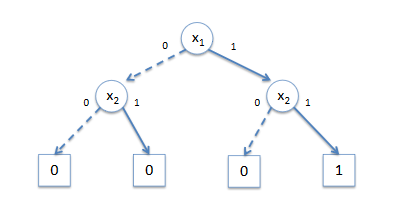
\includegraphics[scale=0.8]{slike/BD_And.PNG}
    \caption{Binarno drvo odlu\v{c}ivanja za funkciju $\wedge$}
    \label{diag:BDAnd}
\end{figure}

\noindent Sli\v{c}no se mogu definisati i ostale korisne funkcije, na primer \texttt{f\_or} ($\vee$) i \texttt{f\_xor} ($\oplus$), sa dijagramima na slici \ref{fig:BDOrXor}:

\begin{lstlisting}[language=C++,escapechar=@]
    bool f_or(bool x1, bool x2) { return x1 || x2; }

    bool f_xor(bool x1, bool x2) {
        return (x1 && !x2) || (!x1 && x2); @\footnote{Ne mo\v{z}emo koristiti operator \^{} jer on operi\v{s}e nad promenljivima tipa \emph{int}, a ne \emph{bool}.}@
    }
\end{lstlisting}

\begin{figure}[H]
    % NE DIRAJ OVE BROJEVE
    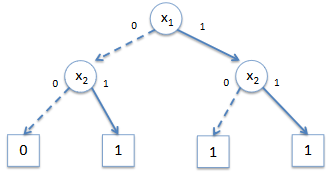
\includegraphics[scale=0.68]{slike/BD_Or.PNG}
    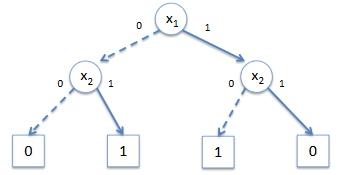
\includegraphics[scale=0.68]{slike/BD_Xor.PNG}
    \caption{Binarna drveta odlu\v{c}ivanja za funkcije $\vee$ i $\oplus$, redom}
    \label{fig:BDOrXor}
\end{figure}

Binarna drveta odlu\v{c}ivanja imaju neke veoma lo\v{s}e osobine. Najve\'c{}i problem je njihova veli\v{c}ina. Binarno drvo za $n$ ulaznih promenljivih \'c{}e imati $2^{n-1}$ unutra\v{s}njih \v{c}vorova i $2^{n}$ listova.

Uprkos tome, postoje i neke dobre osobine, pre svega \emph{kanoni\v{c}nost}. Ukoliko testiramo promenljive uvek u istom redosledu (tada se binarno drvo odlu\v{c}ivanja naziva \emph{uredjeno}), onda je drvo jedinstveno za svaku bulovsku funkciju. Stoga se test ekvivalencije dve bulovske funkcije svodi na testiranje ekvivalentnosti njivohih binarnih drveta odlu\v{c}ivanja. Na\v{z}alost, zbog velikog broja \v{c}vorova u drvetima, problem je eksponencijalne slo\v{z}enosti u odnosu na broj ulaznih parametara.

Kako bi se re\v{s}io problem eksplozije broja \v{c}vorova u drvetu, formiraju se unapredjenja binarnih drveta odlu\v{c}ivanja - binarni dijagrami odlu\v{c}ivanja (\emph{BDD}). O njima \'c{}e biti vi\v{s}e re\v{c}i u poglavlju koje sledi.
